\documentclass[a4paper]{article}
\usepackage[utf8]{inputenc}
\usepackage[english]{babel}
\usepackage{url}
\usepackage{graphicx}
\usepackage{array}
\usepackage{geometry}
\usepackage{tabularx}
\usepackage{pgfplots}
\usepackage{amsmath}
\usepackage{amsfonts}
\usepackage{amssymb}
\usepackage{placeins}

\title{Intelligent Patient Record}

\author{ITU \\
\vspace{5mm}
Mathias Schmidt, Thomas Snaidero \\
Supervisors: \\
Steven Houben, Mads Frost}

\date{21 May 2014}

\begin{document}

\maketitle
\pagebreak
\tableofcontents
\pagebreak


\section{Introduction}

A physical patient record consisting of a folder and papers, has a wide presence in hospitals. It is used daily by doctors and nurses who share it with each other, as each patient has one record bound to them. It has remained physical (as opposed to digital) for many reasons, some of them being that paper holds legal value, and hospitals often rely on a large IT infrastructure that is hard to update and modify, due to legacy software and databases that have become hard to maintain due to their old age. Hospitals have since adopted a double record, consisting of a physical and a digital part. \\

A recent article by Houben et al. proposed an enhancement of such a double record, dubbed the Hybrid Patient Record (HyPR), to resolve configuration problems related to finding, using and managing the physical and digital representation of the patient record. A device prototype was created, to merge the physical and digital patient record
into one physical enclosure. A study with clinicians pointed toward a will to adopt such device, but the weight, thickness and size were deemed to be a very important factor \cite{hypr}. \\

In this project, an improvement of the physical part of the Hybrid Patient Record is proposed. As the original device by Houben et al. was an early prototype, the design, size and choice of materials were assessed, and modified. With the availability of prototyping tools at the IT University of Copenhagen, such as a laser cutter and 3D printer, the method of rapid prototyping was therefore chosen for developing a new device. Through an iterative process, a series of prototypes were created and evaluated. 

\clearpage

\section{Brief description of the features}

The Hybrid Patient Record can enhance a paper based patient record in many ways. It attempts to achieve that, through the addition of a small microcontroller that makes it possible to control LEDs, a small speaker, an RFID reader, and WiFi connectivity. \\
For instance, the record is often lost or misplaced both inside the ward or in other departments of a hospital \cite{hypr}. The HyPR device is then equipped with an ultrasound tag that broadcasts a unique value, and makes it able to be tracked down to a specific location in the hospital. A small speaker adds an identification sound for the device, and allows it be found if it is lost in a room. \\
LEDs can show a colour scheme. The colour can, for example, represent a specific nurse, a patient status or simply used in combination with sound to identify a specific device in a stack of patient journals. \\
An RFID reader reads a tag from a doctor's tablet, so they can quickly access relevant data for the associated patient. \\
WiFi capability is added in order to be able to for example, change the LED colours, or trigger the speaker.

\section{Design requirements}

Numbered list of product requirements with most important first, least important last.

Physical requirements
- lightweight
- small / thin
- maintainability 
	- quickly upload new sofware
	- as close to pick and place as possible
	- easy to change components

Electronic requirements
- rechargeable battery via standard USB cable
- battery status
- long autonomy 
- easy to see LED colours from distance
- easy to hear the audio signal
- ability to connect to wifi
- ability to red RFID tags
% Numbered list of product requirements with most important first, least important last.

%\section{Use case scenarios}
Detailed description of 3 use case scenarios which illustrate:
- The user experience
- Insight about a specific product feature, or user requirement
% Detailed description of 3 use case scenarios which illustrate:
% - The user experience
% - Insight about a specific product feature, or user requirement

%\section{Design analysis and concept diagrams}
Description of issues related to the design of the product:
- Description of concepts, requirements and features of the product
- Review of motivations for making the design decisions
- Indicate the primary features of the design that are the most creative and original
% Description of issues related to the design of the product:
% - Description of concepts, requirements and features of the product
% - Review of motivations for making the design decisions
% - Indicate the primary features of the design that are the most creative and original

\section{Materials}
\subsection{Plastic for lasercutting}
For this project we got a bunch of different plastic materials from RIAS, in order to find some material that might be cheaper, and better that acrylic, since acrylic have tendency to be brittle, this becomes worse when it has been laser cut.
all of the plastic was thermoplastic, which is a term that is used in the laser industry to indicate that it can be laser cut.
For the laser cutter we made some simple figures to see what the result would be.
The requirements for the material is that it is easy to lasercut, and don't break easy.
\subsubsection{PEHD}
The first material that we tried to cut was, PEHD which is used in the production of ex. plastic bottles and corrosion-resistant piping it is known for having a high strength to density ratio.
The cutting went fine, but there was some residue left over from the cutting, that we had some problems removing.
% There ware some problems getting the resedu off the plastic after the cutting, also the material have a tendensy to hold it's form when bent.%
\begin{figure}[!h]
	\centering
	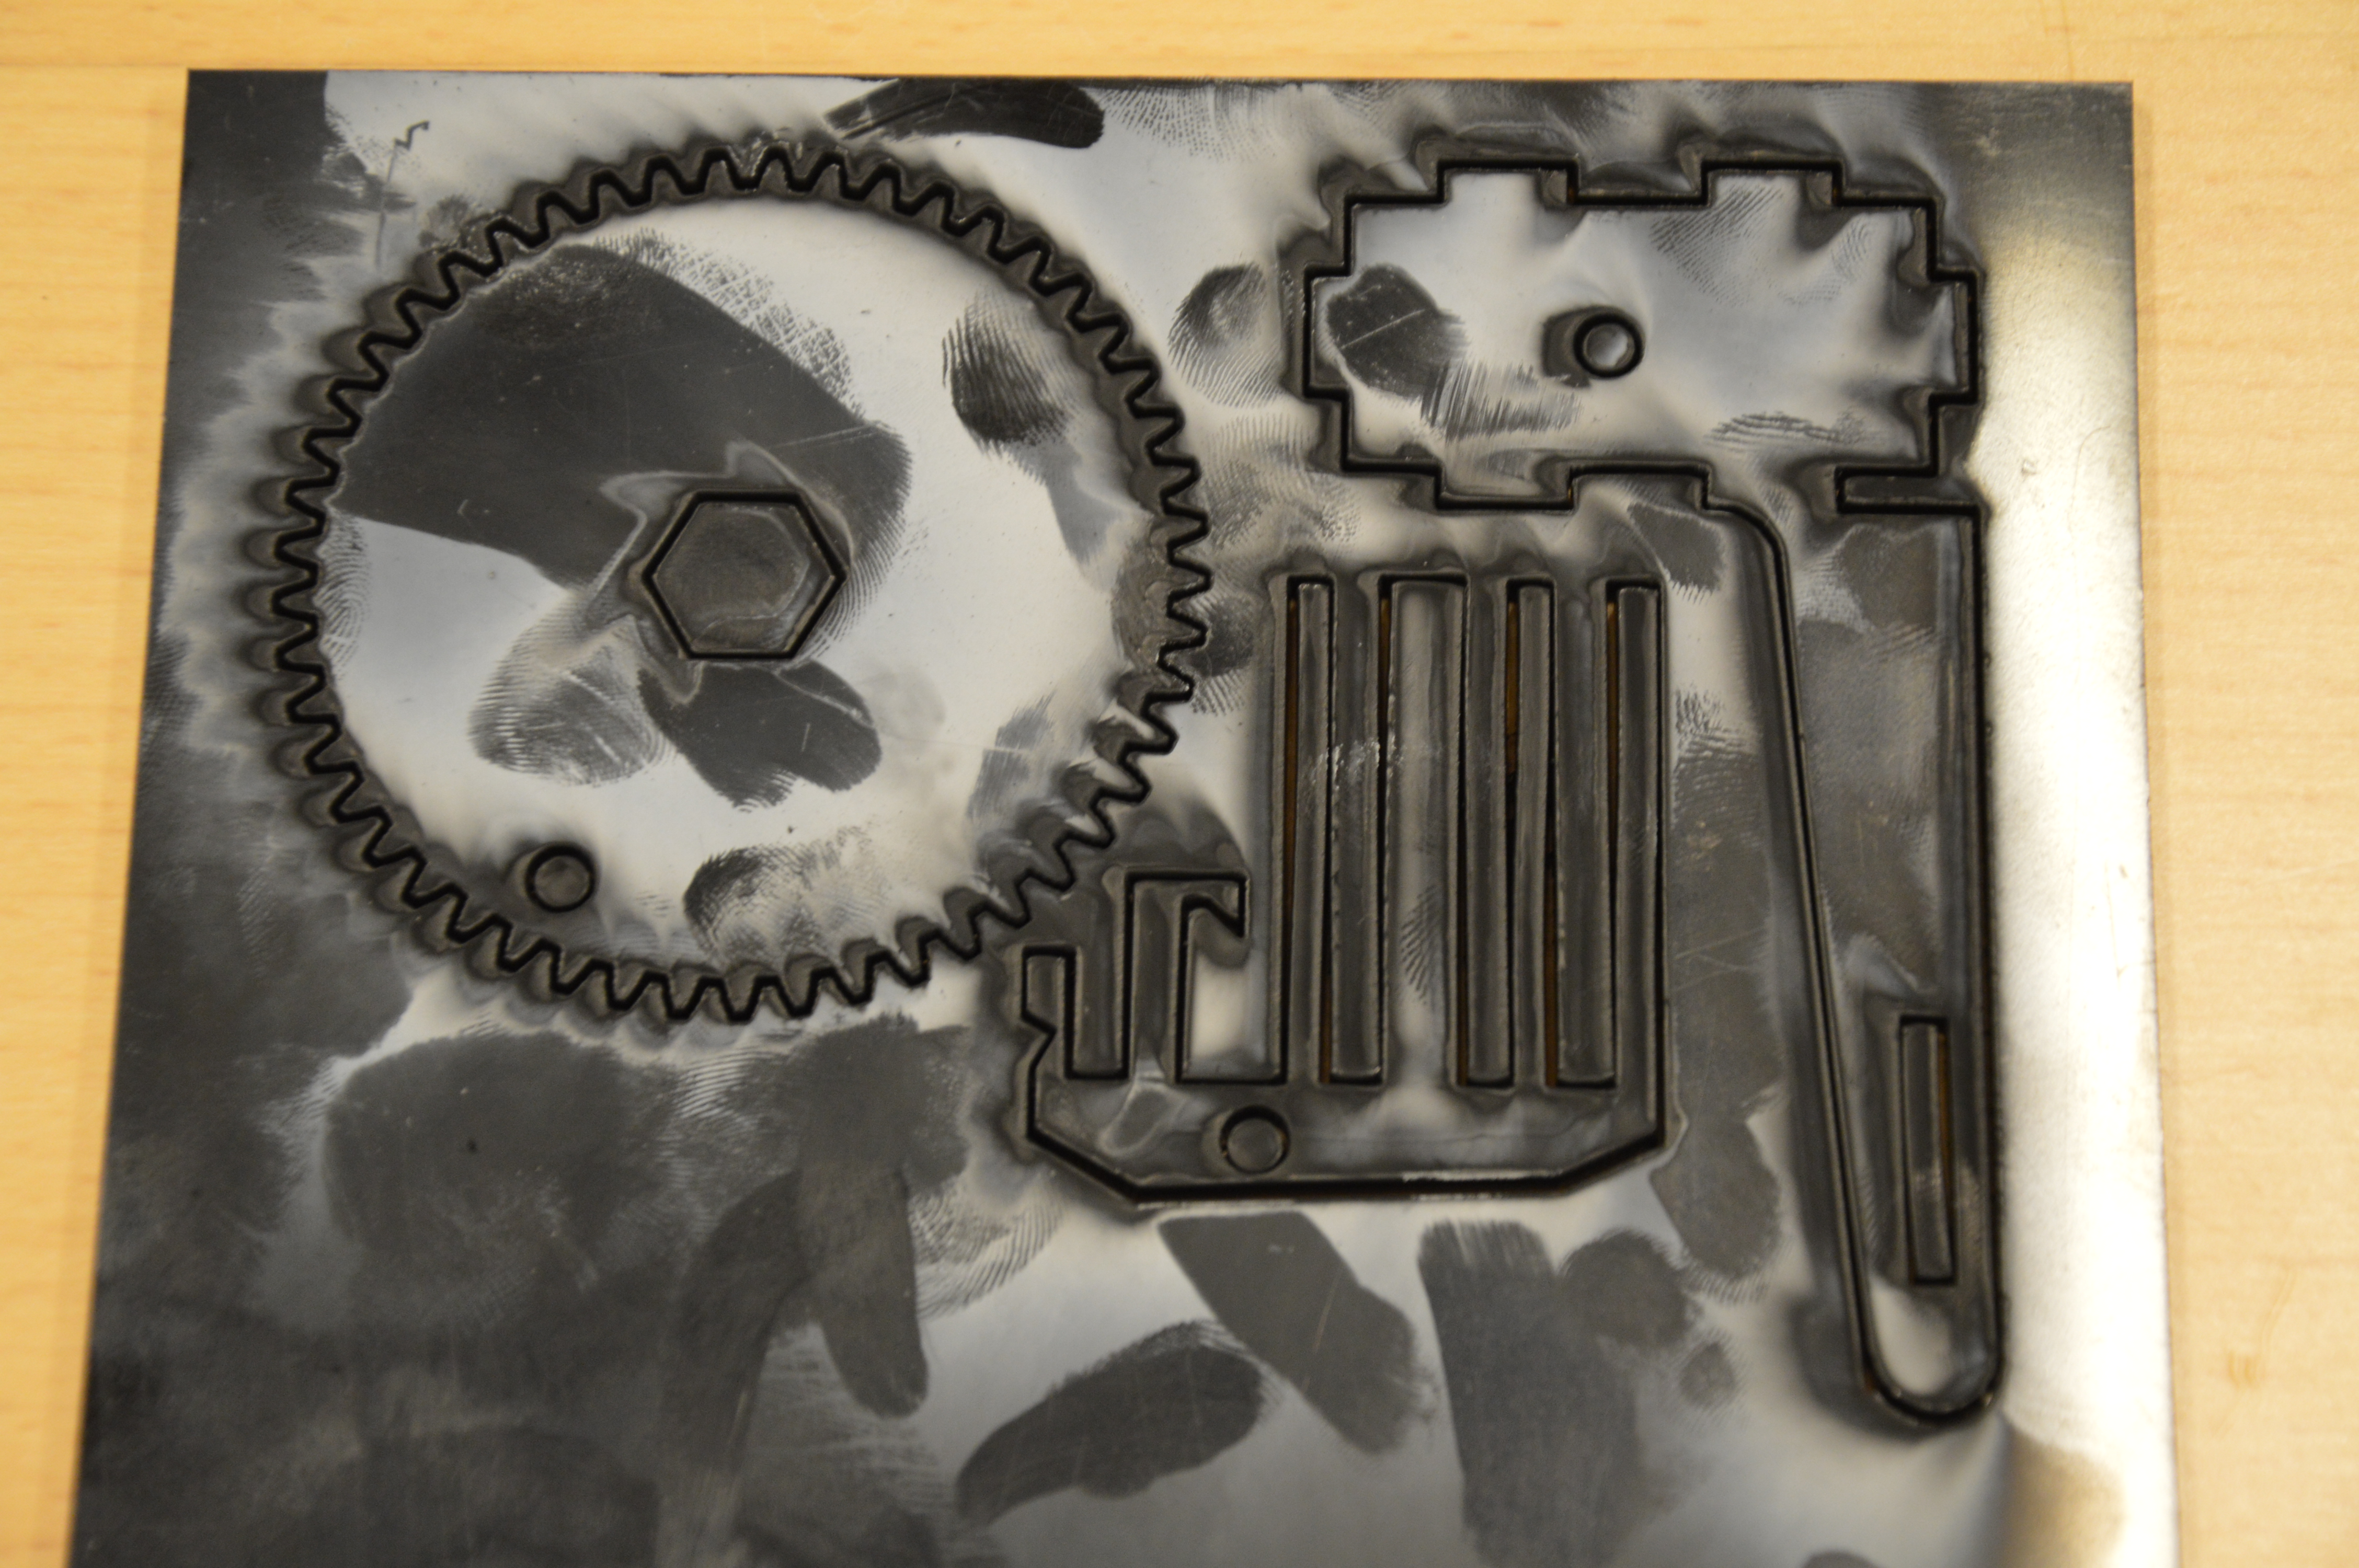
\includegraphics[scale=0.1]{images/DSC_0048.JPG}
	\caption{\small {\it {Cut test of PEHD}}} \label{fig:PEHD}
\end{figure}
\FloatBarrier
\subsubsection{ PP}
 PP is most commonly used in packaging and labeling, and it has resistant to many chemical solvents, bases and acids.
The cutting had some big problems, one of them was that after 3 cutting rounds, the laser still haven't cut through the material, which meant we had to let it be, and not trying to cut in that material.
\begin{figure}[!h]
	\centering
	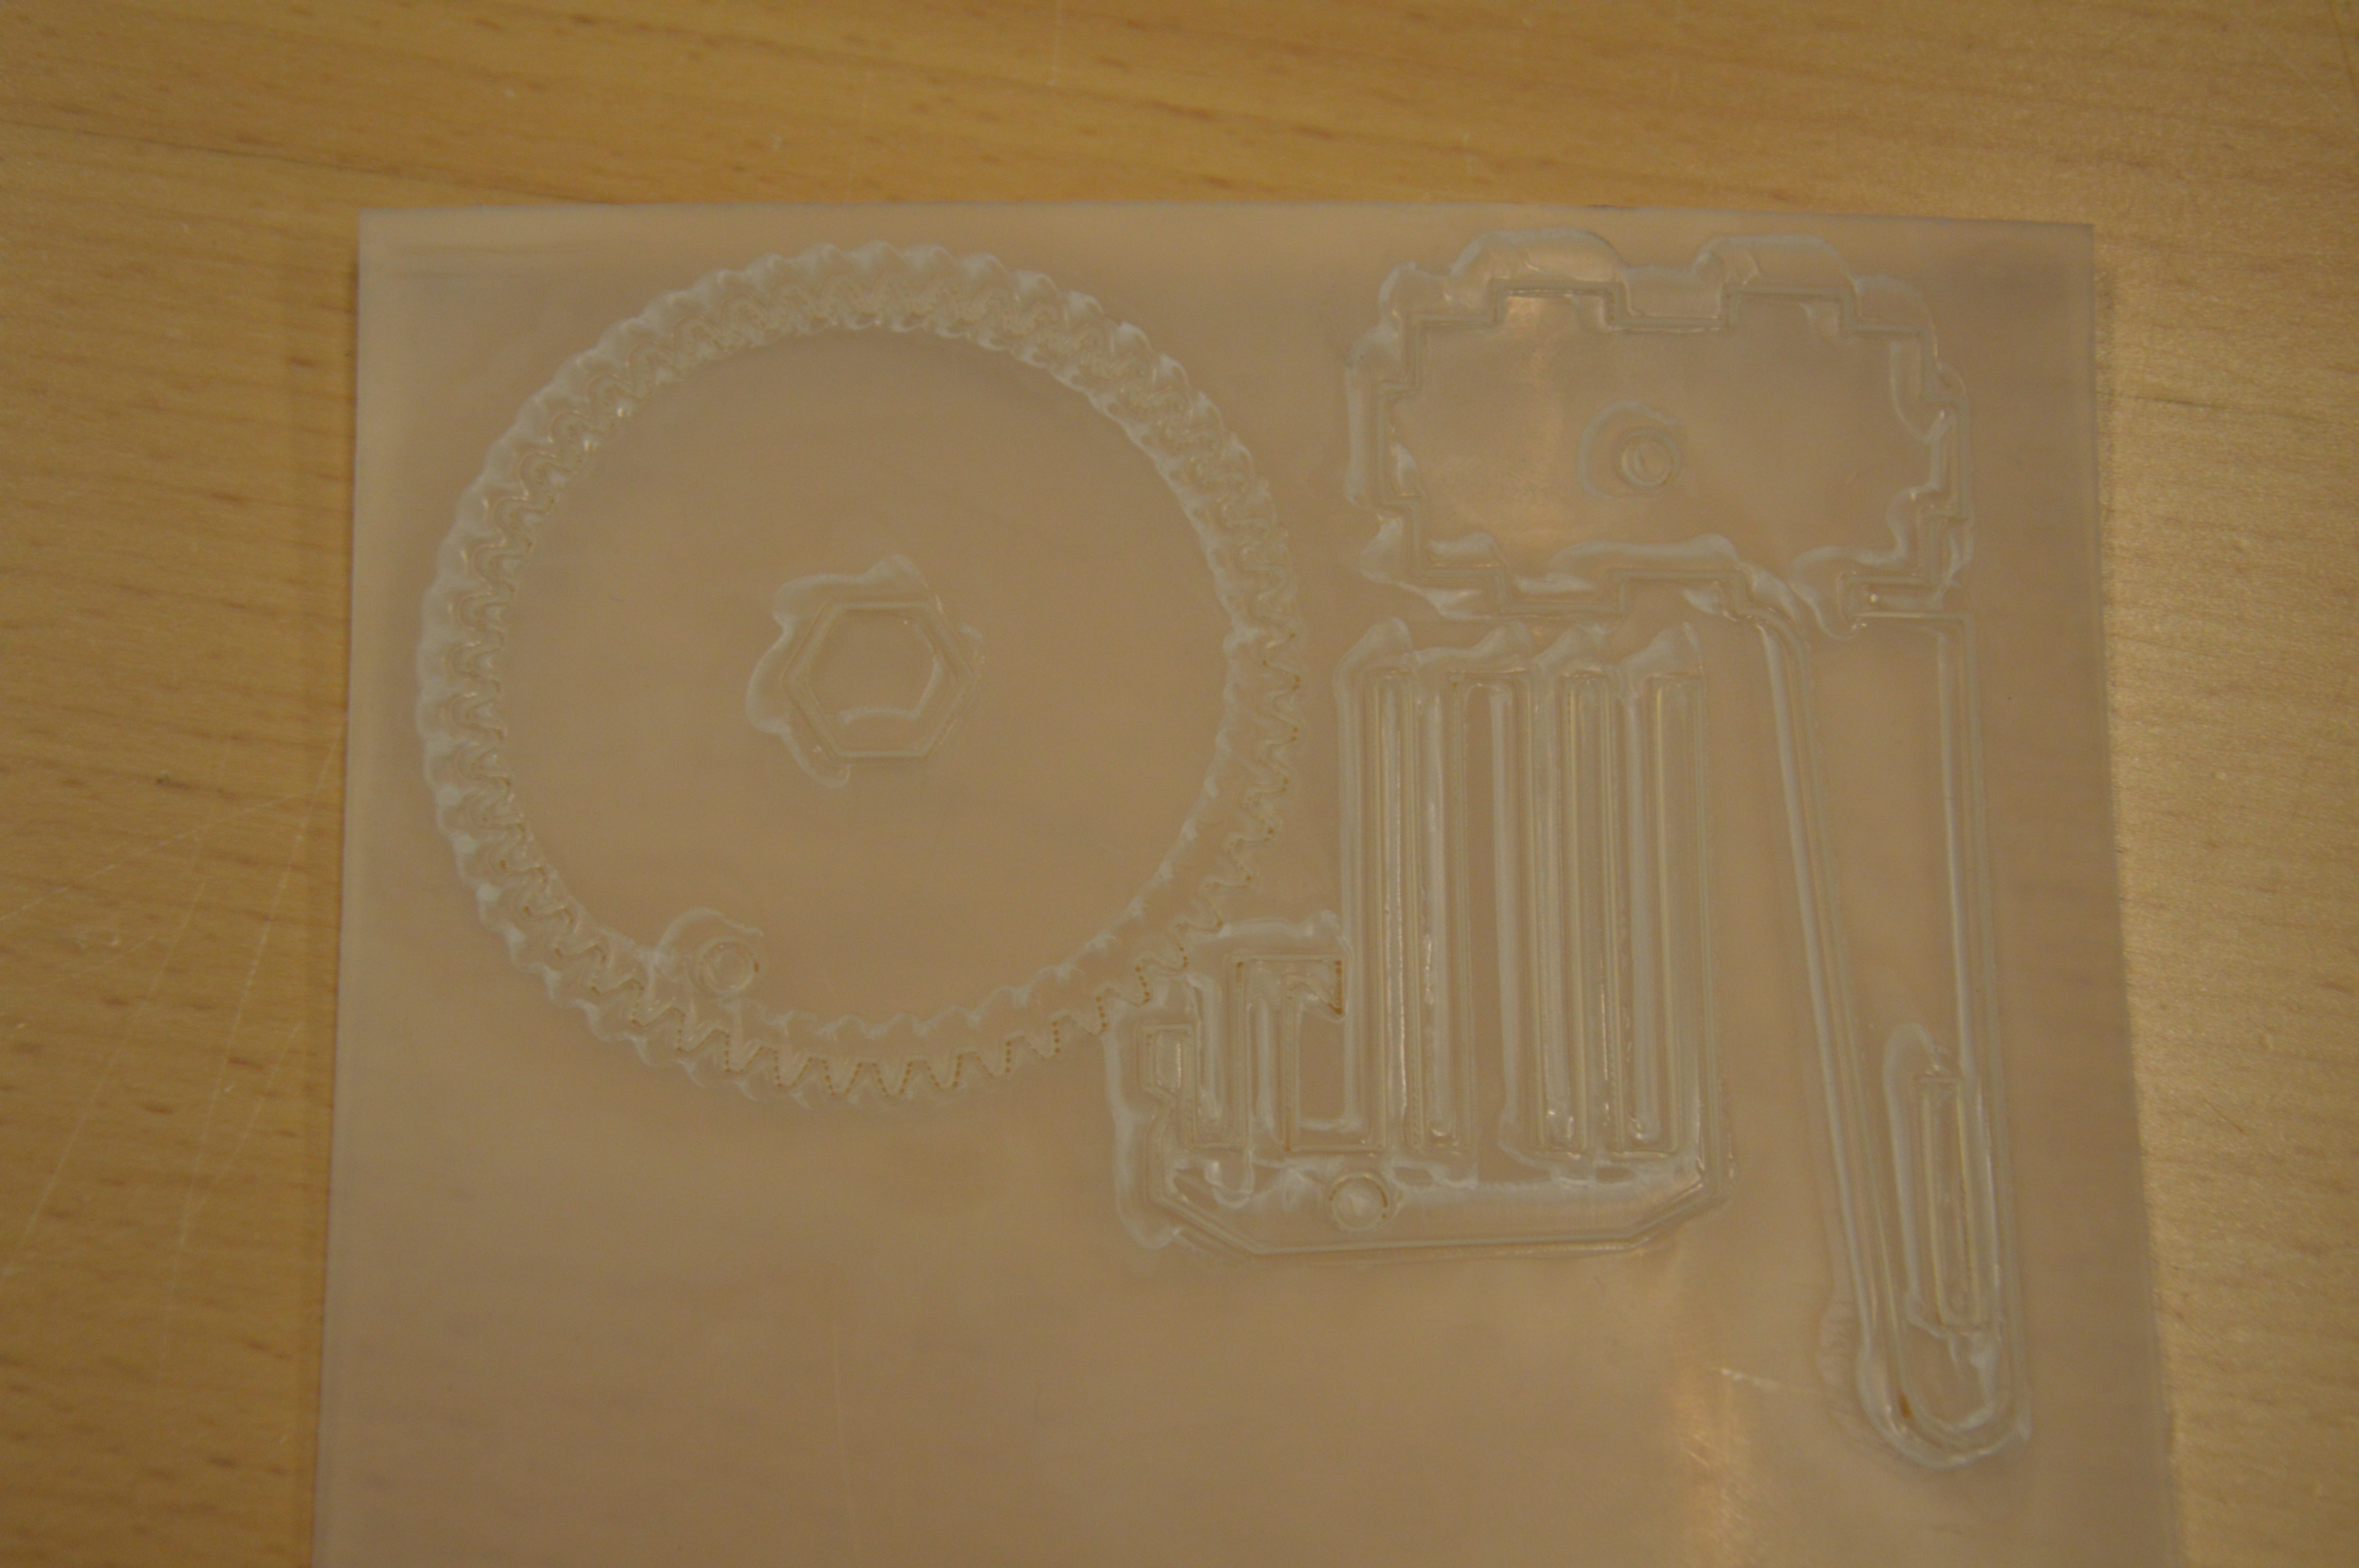
\includegraphics[scale=0.1]{images/DSC_0053.JPG}
	\caption{\small {\it {Cut of RIALEN PP}}} \label{fig:PP}
\end{figure}
\FloatBarrier
\subsubsection{PP-H}
Is PP where they have added Homopolymer to, this changes the materials propertyes, so it is becomes easier to cut, but it leaves some residue when cut, it also have tendency to curl up on it self, where it has been cut.
However the material has memory, which means that it remember the shape is has been bend, this is a problem since we are going to have some eletronic attach to it.
\begin{figure}[!h]
	\centering
	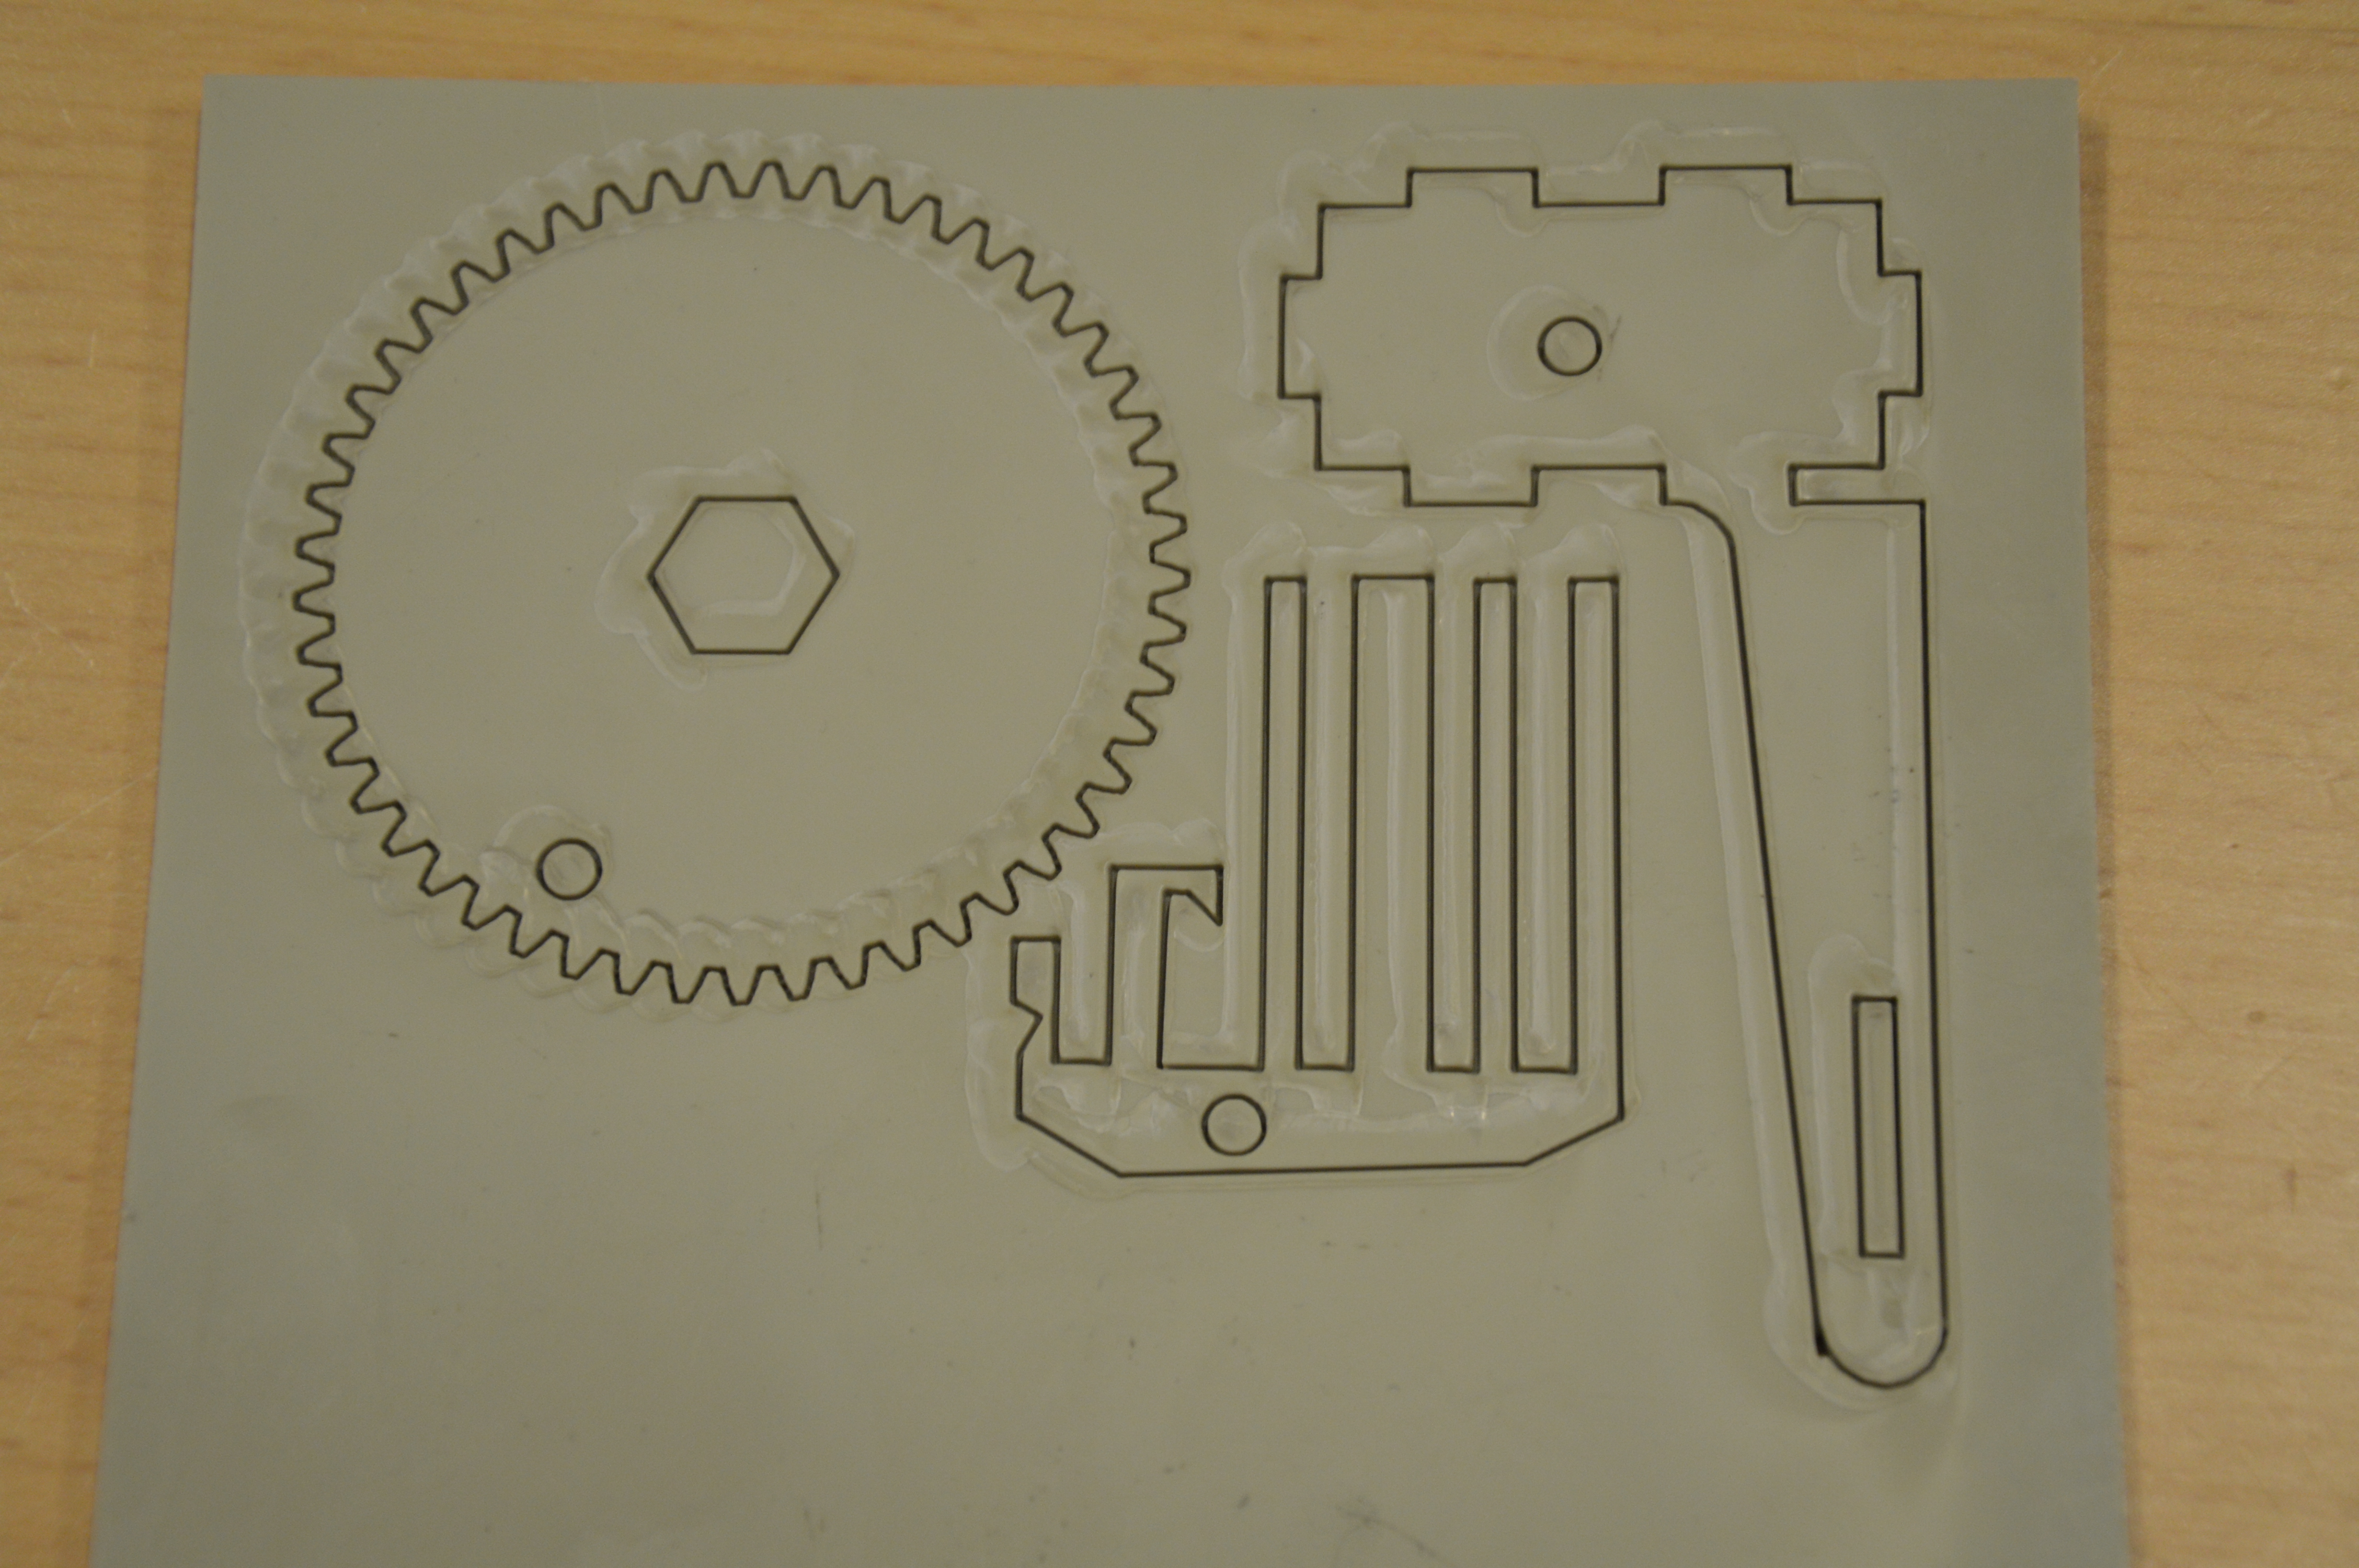
\includegraphics[scale=0.1]{images/DSC_0029.JPG}
	\caption{\small {\it {Cut test of PP-H}}} \label{fig:PP-H}
\end{figure}
\FloatBarrier
\subsubsection{PETG}
PETG is used alot in the production of plastic bottles, and is a durable material.
The cutting process did not go as hoped, be side that one can see the burn marks, it also had a very strong chemical smell, that took weeks to dissipate.
\begin{figure}[!h]
	\centering
	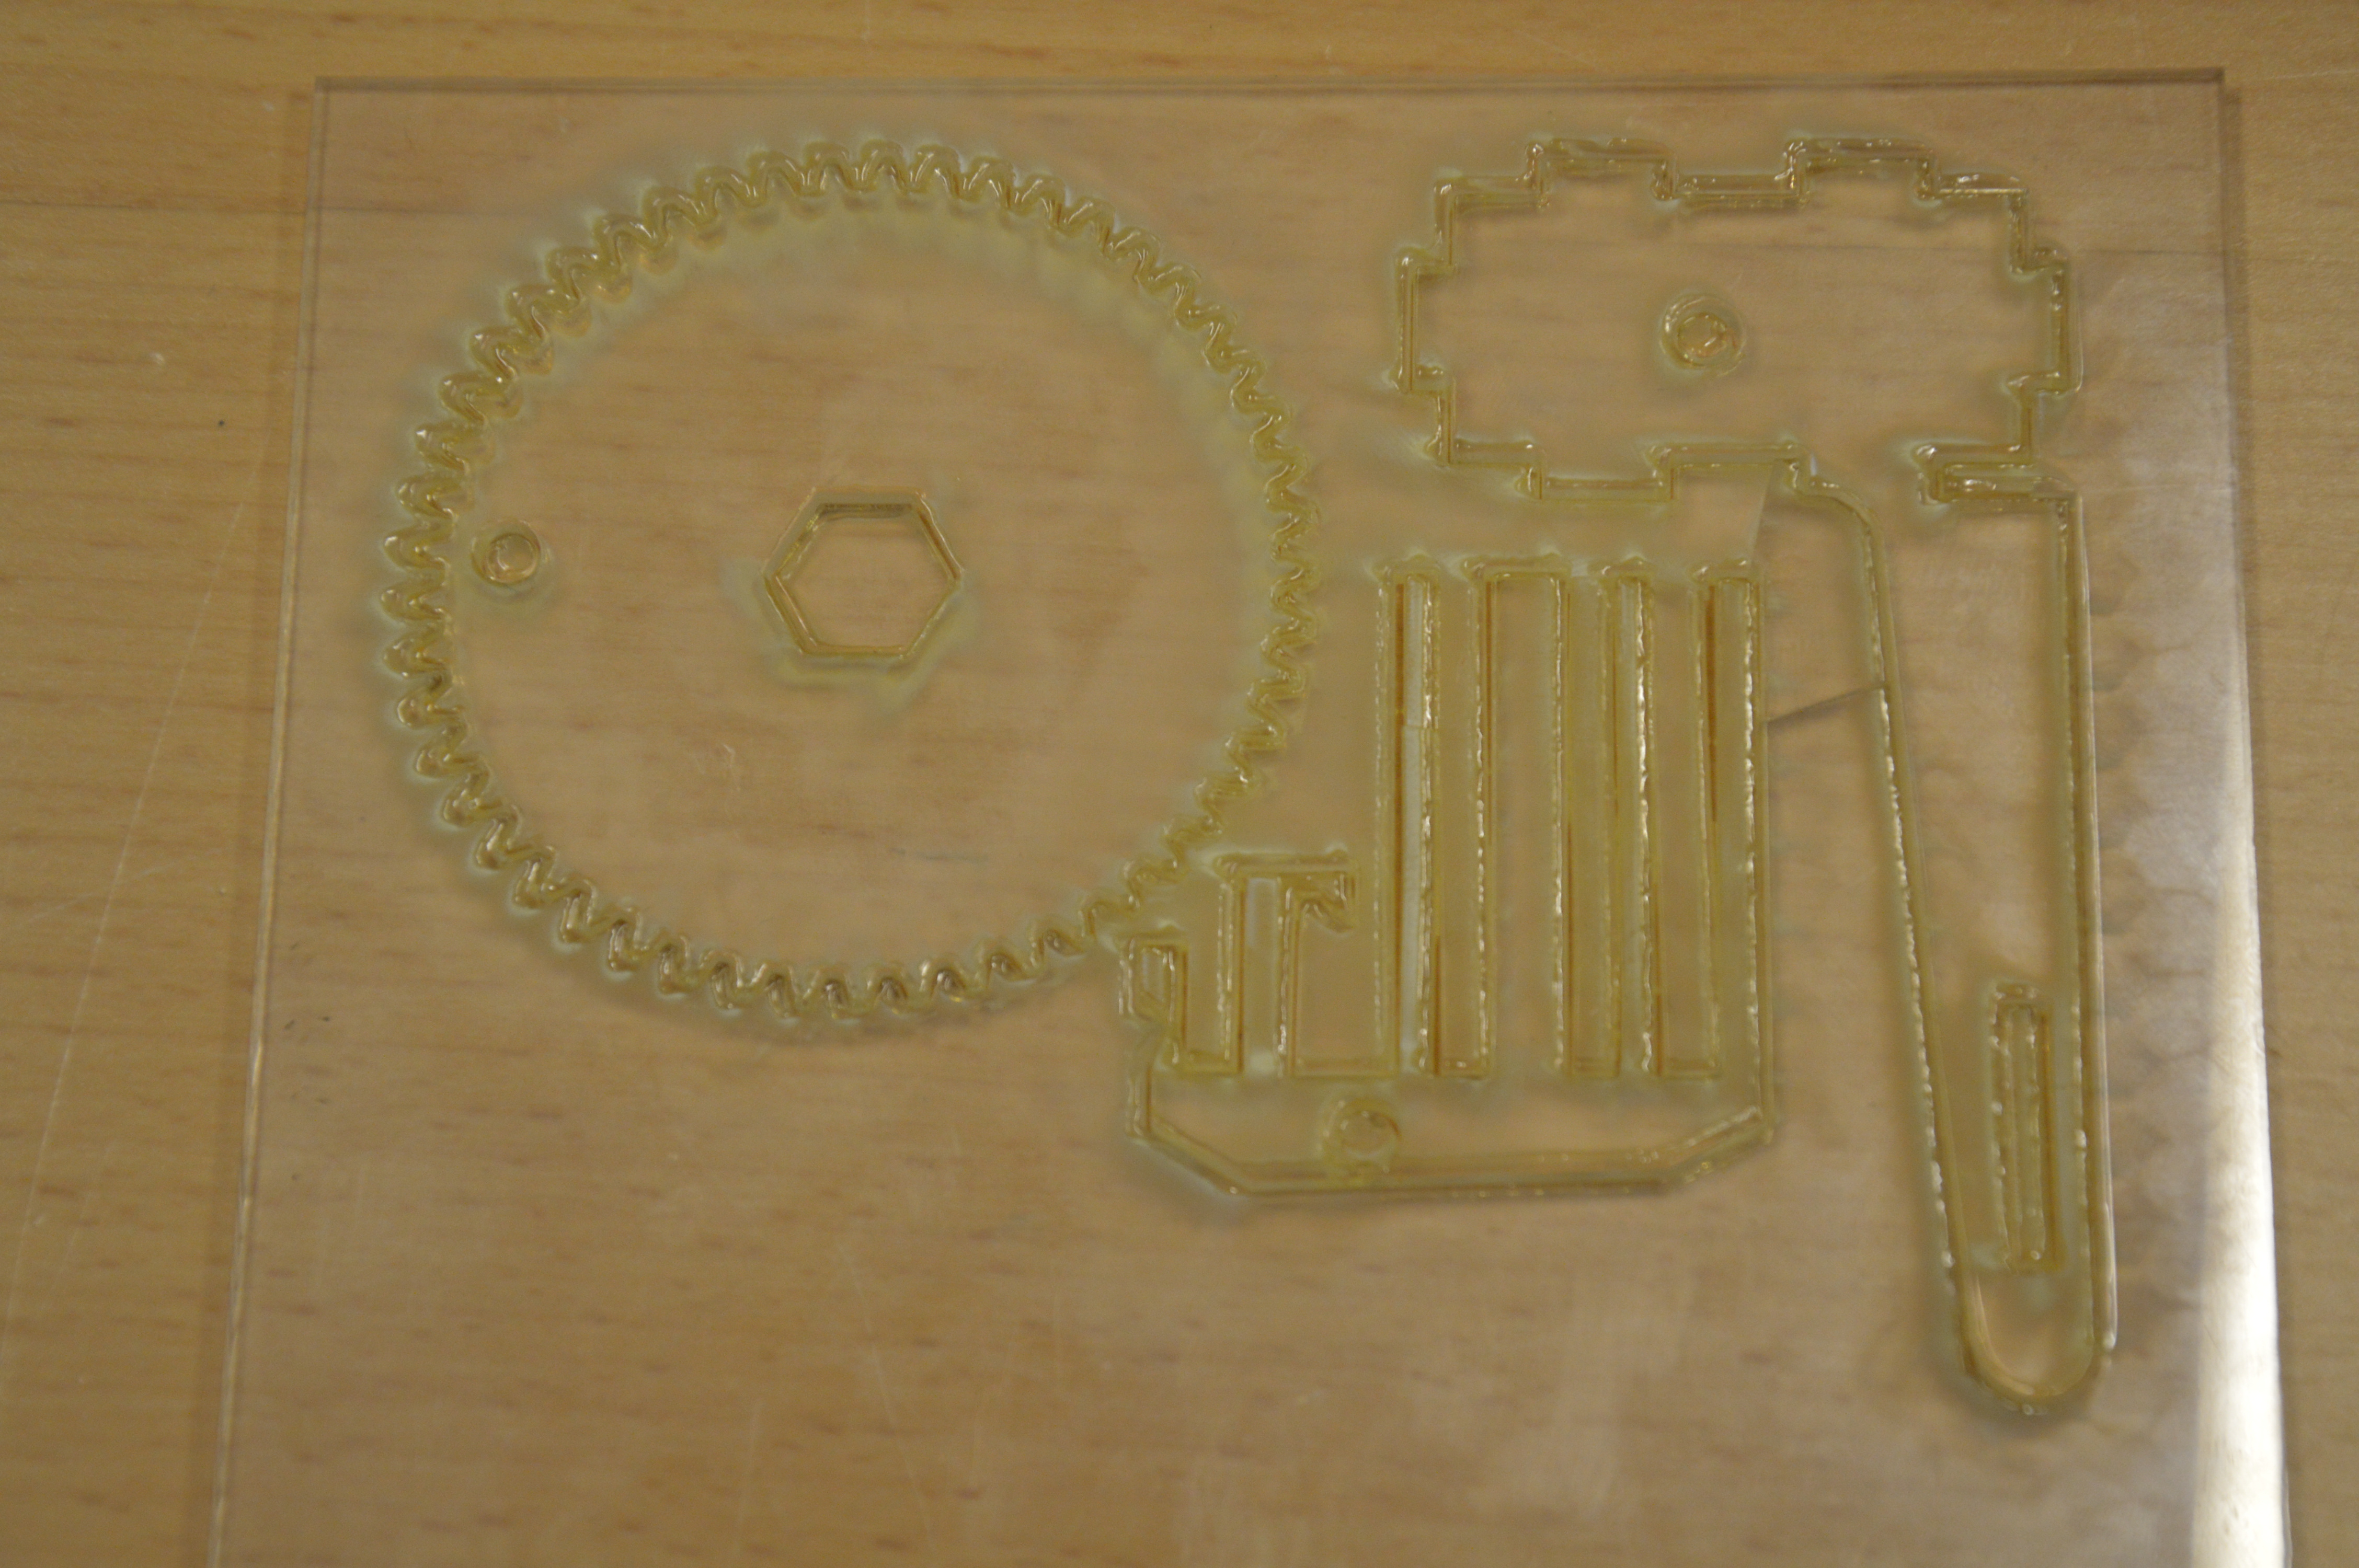
\includegraphics[scale=0.1]{images/DSC_0023.JPG}
	\caption{\small {\it {Cut test of PETG}}} \label{fig:PETG}
\end{figure}
\FloatBarrier
\subsubsection{POM-C}
POM-C is a material that works well with laser cutting, it is used commonly in small gear wheels, ball bearings, and many other product where you need low friction and stiffness.
The cutting of it went fine, but we found out that if we want to use it, we may have some problems since the glue, that is used for it is highly toxic, furthermore the material more expensive compared to Acrylic.
\begin{figure}[!h]
	\centering
	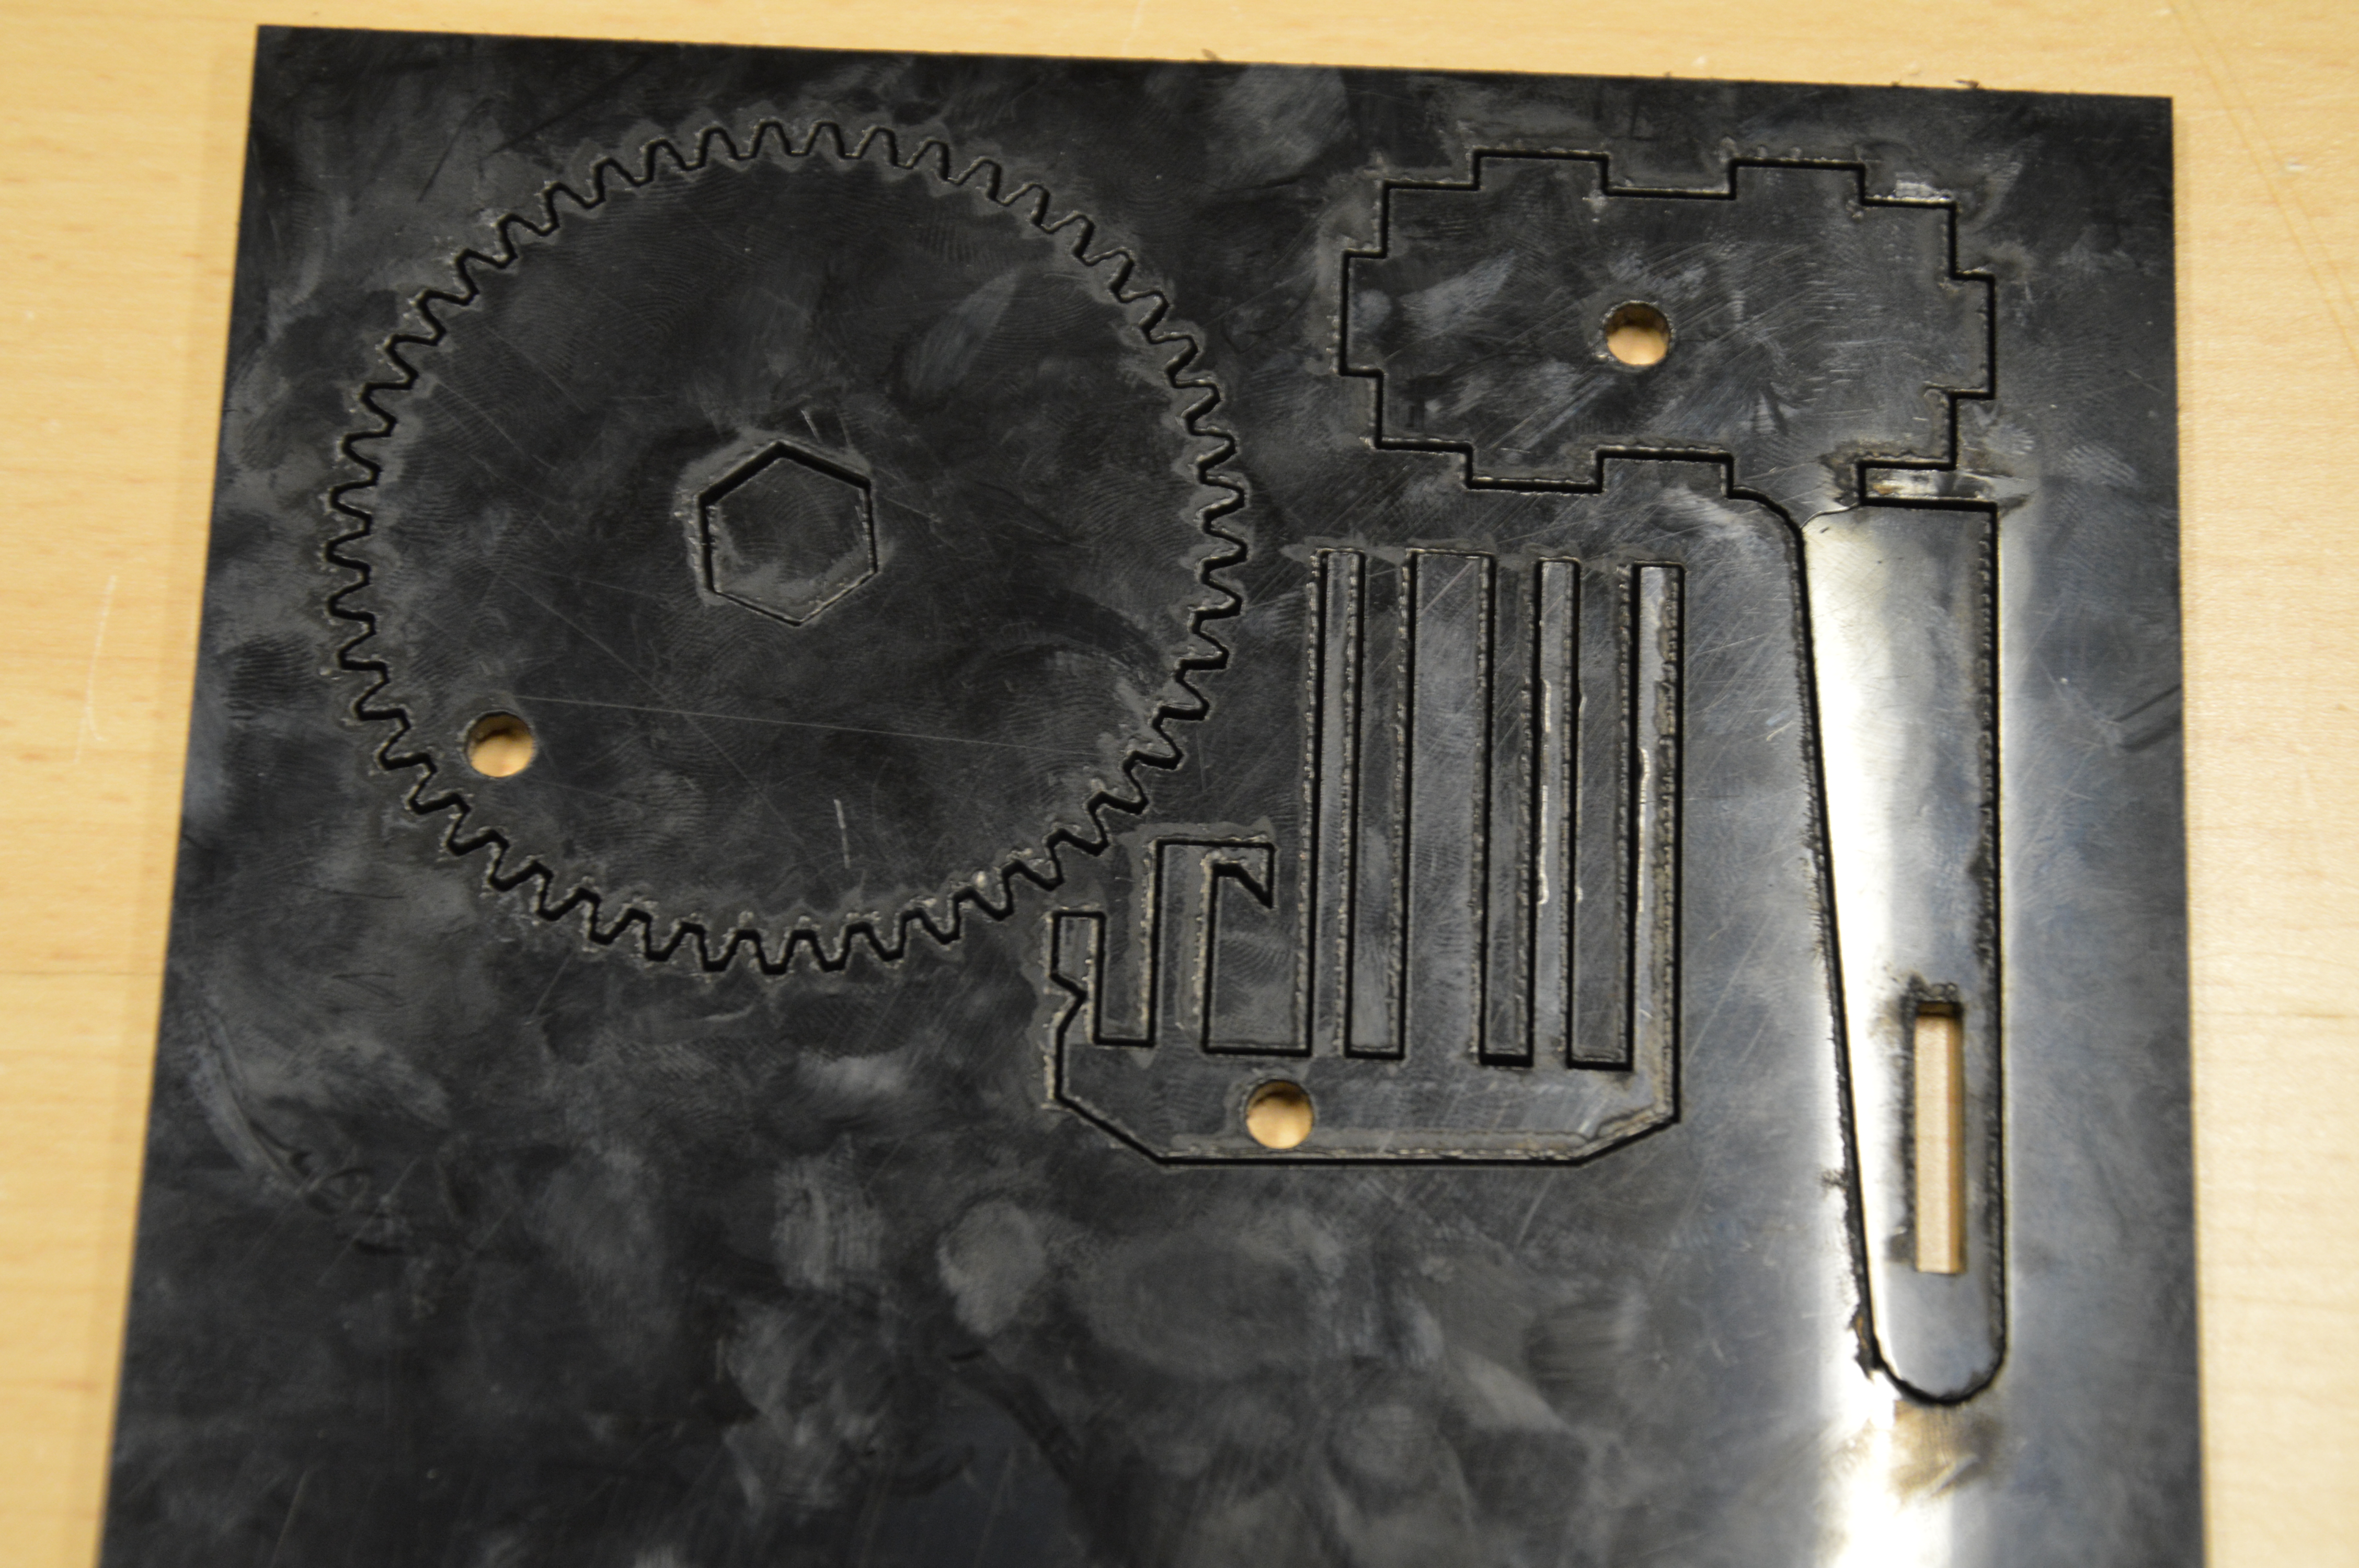
\includegraphics[scale=0.1]{images/DSC_0039.JPG}
	\caption{\small {\it {Cut test of POM-C}}} \label{fig:POM-C}
\end{figure}
\FloatBarrier

\subsubsection{PEEK}
PEEK is one of the materials that we would have liked to try out since it is one of the materials that are used in the medical industry, however it is an expensive material and it is hard to get in sheets, we did have some conversion over mail with RIAS, but was unable to secure some samples.

\subsubsection{ACRYL}
Acrylic is a easy material to use in a laser cutter, the biggest problem with it, is that it is brettle, and does have a tendency to break when it hits something hard or comes under tension.
we did not try to make test cuts in it, since we have cut a lot of acrylic and know the properties of it.


\subsubsection{Conslusion}
The conclusion is that we are going to use acrylic, since we have easy accesse to it and it's cheap, and can try to mend the disadvantages.

\subsection{Plastic for 3D printing}
There are 2 commenly used plastic for 3D printing PLA and ABS

\subsubsection{PLA}
PLA (poly lactic acid) is a bio-degradable plastic that is mostly made from corn starch or sugar cane.
It has a lower melting point that ABS, and can be printed on a cold surcafe. you can also print faster with highere presision. you don't need a ventelated room like abs, since it does not produce plastic fumes. And it is food safe.

However it is less sturdy, have a shorter lifespan that ABS. Since it has a lower melting point that ABS it can deform when heated Ex. hot water will deform it.

\subsubsection{ABS}
ABS (Acrylonitrile Butadiene Styrene) is made from oil, and has a highere melting temperture than pla, it also have highere strength and flexibility and a logerlifespan, which is the reason that it is used in Ex. LEGO

It does have some downside, it deformes when you don't print in on an hot surface, which makes it harder to print. It gives out plastic fumes when printed, so you need a ventilated room, and it is not suitable if you going to use it with food.

\subsubsection{Conslusion}
We have chosen to use PLA, since the printers that we have are using it and the rooms they are in arn't ventilated.

http://www.protoparadigm.com/blog/2013/01/the-difference-between-abs-and-pla-for-3d-printing/

\section{Theory}
\subsection{Rapid prototyping}

Prototyping of a physical product is an age old process that has evolved all the way to today. Up until the emergence of virtual prototyping with CAD applications, prototyping was manual, and tended to be craft-based, thus very slow \cite{chua2010}. \\
In the 1980s, virtual prototyping became more widespread, as computer tools became more mature. Virtual models could now be analysed and modified as if they were physical prototypes, and several iterations of designs could be easily carried out. But as the prototypes became more complex, the time required to make a physical model increased, and therefore craft-based production of a physical prototype became tedious \cite{chua2010}. \\

A new type of prototyping has therefore emerged in the 1980s, called rapid prototyping (RP). Rapid Prototyping can be defined as techniques used to quickly fabricate a scale model of a part or assembly, using three-dimensional computer aided design (CAD). \\

Rapid Prototyping has also been referred to as solid free-form manufacturing, computer automated manufacturing, and layered manufacturing \cite{efunda}. An RP model's most used scenario is for testing various qualities of a physical product, and in some cases, the RP part can be the final part, but typically the RP material is not strong or accurate enough. \\

There exists many experimental RP techniques such as Stereolithography (SLA), Digital Light Processing (DLP), Laminated Object Manufacturing (LOM), Electron Beam Freeform Fabrication (EBF3), Fused Deposition Modelling (FDM), and more \cite{wiki3D}. The latter was specifically used in this project, because of its almost ubiquitous presence in universities, fab-labs, and hackerspaces. \\

The main reasons for using Rapid Prototyping are very compelling. It decreases costly mistakes and engineering changes, thus minimizing development time. By being able to have a look at the product early in the design process, mistakes can be corrected, and changes can be made while they are still inexpensive. \\

Rapid prototyping can be performed in many different ways, but they all adopt the same basic methodology:

\begin{itemize} \itemsep0em
  \item A virtual model is designed in a CAD application.  It represents the part that is physically built as an enclosed volume, and will specify the inside, the outside, and boundaries of the model.
  \item The model to be built is next converted into an STL (Stereo Lithography) file format. The STL format approximates the surfaces of the model by polygons.
  \item A program analyses the STL file, and ``slices'' the model into cross-sections. It generates paths to be filled and calculates the amount of material to be extruded, in the case of a 3D printer that uses fused deposition modelling \cite{slic3r}. In short, it converts a digital 3D model into printing instructions for a 3D printer.
  \item The model and any supports are removed. The surface of the model is then finished and cleaned for imperfections \cite{efunda}.
\end{itemize}


\section{Building process}
\subsection{Software}



% For the Design we have used openscad, and steard away from 3d design programs like 3d studio max and blender.
% The reason is when you design a file in 3d studio max or blender, it might look big, and you may have followede the messurments in the program, you usual have to multiply the figur by a factor of 1000x due to conversion problems. Beside that you can have problems with the node points in the design, some times the design file might lock like all the points that need to be conected are, but when you multiply the figure by a factor or zoom up close, that might not be true, and that can give problems.
% The othere is the avalibity and price, openscad is a simple, lightwitght and opensource program that is easy to learn and use for programmers, since you create objects if by writing simple code ex. Cube([5,5,5]); 
% We could have bought a linces for some other program like autocad or different cad program, but we found the unessery since it is simple 3D models, and we don't need a huge program for that.

% When the design is done we have exportede the openscad file to STL, that we have but into scli3r, that are one of the best stl to gcode convert there exsist, where you take stl files that are exportede from openscad and convert them to gcode, which is instruction code that the firmware on the 3D printer understand. beside that it is openscource, and is used for almost all 3d printeres.

% For the laser cutting we have used inkscabe, which also is an opensource program, the reason is that we only had to change the line thickness on the DXF file that was exported from openscad. and save it as an pdf. 

% \subsection{Machines}
% \subsubsection{3D Printers}
% There is a lot of different 3D printers design, the printers that we had access to was prusa i3 at ITU, and MAXbot in labitat, they work in the same way, with it's x,y  and z axsis, the main differense is the thickness of the pla that they use, geearing and how the bed is cunstructed. The prusa i3 at ITU usses 3mm pla vs MAXbot that uses 1.75 mm pla, this has the complecation that prusa need to have a gearing system in order to give enough pressur.
% The last main difference is that the Prusa i3 don't have any springs in the bed, which can leed to some problems where the nossel get attach ot the print and force it of the plate.

% \subsubsection{Laser cutter}
% For the laser cutting we have used the 60W laser at ITU, we did have some back up at some different fablabs, if the laser stop working.

% \section{Design specifications}
% Explanations of how to build the product, including information such as:
% - System architecture
% - Drawings and sketches
% - Parts and supply ordering information

% \subsection{Hardware}
% Arduino
% Wifi
% RFID
% Buzzer
% Led
% Capicitor
% Battery
% Battery charger

\section{Prototyping analysis}

Discussion of experience in building prototypes during the design process:
- Illustration of all the prototyping activities
- Discussion of specific areas where the experience of building prototypes affected the design requirements and specifications
% Discussion of experience in building prototypes during the design process:
% - Illustration of all the prototyping activities
% - Discussion of specific areas where the experience of building prototypes affected the design requirements and specifications

\section{Design specifications}
Explanations of how to build the product, including information such as:
- System architecture
- Drawings and sketches
- Parts and supply ordering information

Design specifications marked for:
- Quality
- Accuracy
- Originality
% Explanations of how to build the product, including information such as:
% - System architecture
% - Drawings and sketches
% - Parts and supply ordering information

% Design specifications marked for:
% - Quality
% - Accuracy
% - Originality



\section{TESTING - ignore}

\begin{figure}[h]
\begin{center}
\includegraphics[scale=0.5]{figures/explode.png}
\caption{\small {\it {This is a description}}} \label{fig:explode}
\end{center}
\end{figure}

\clearpage

\section{Conclusions}

This report has presented the detailed design process of a hardware device. Whether the device fulfilled its purpose or not, was not entirely the intent of this report, but to document the series of steps to come up with a solution to a problem. The solution involved designing a product (an intelligent patient record prototype) that meets certain criteria and accomplishes certain tasks. \\

The report documented the use of the engineering design process, and what methods were chosen for each step. Brainstorming was used for idea generation, and choosing possible solutions. Different kinds of prototyping methods were described, with a focus on rapid prototyping. Evaluation methods such as thinking-aloud was used in order to give inspiration for a new possible brainstorming session. \\

The project has been very enriching, with regards to how a product is designed and prototyped. With the recent emergence of the popularity of cheap 3D printers, rapid prototyping using fused deposition modelling has been made possible here, where it was before only available in the domain of companies with much more resources than a hackerspace. This made it possible to create an open, high-fidelity prototype for evaluation.
 


\clearpage

\bibliographystyle{plain}
\bibliography{References}



% \input{Electronic.tex}

% \section{Design}
\subsection{Materials}
We got a bunch of different plast materials from RIAS, in order to find some material that might be cheaper, and better that acrylic, since acrylic have tendency to be brittle, and this becomes worse when it has been laser cut. 

\subsection{Iterations}
we have used prototyping in order to get a viable device, through the different designs we have been able to see different problems, which have ment that we had to iterate to a new version, we have been limited by time, so we have had to make some compromises

\subsubsection{fisrt}
The first iteration that we build did have some problems.
The first is that it is expensive to build, since we are using a lot of acrylic, the secound point is that it still is heavy, and unwieldy.
But i did give some ideas for the next iteration.

\subsubsection{secound}


\subsubsection{thried}


\subsubsection{fourth}


\subsubsection{fith}



% \input{Problems.tex}








\end{document}


%-----------------------------------------------
% Resources

http://www.me.umn.edu/education/undergraduate/writing/How-to-write-a-Design-Report.pdf

http://pastebin.com/raw.php?i=xudGnU7U

http://ocw.mit.edu/courses/sloan-school-of-management/15-783j-product-design-and-development-spring-2006/index.htm

